\chapter{Computing Prefetch Lookahead for Critical Loads}\label{Chapter4:Methods to predict Look ahead depth for critical delays}
Having decided the set of critical loads in the last chapter, we now turn to discuss the algorithm for run-time determination of prefetch lookahead of these loads. We incorporate our algorithm into SPP.

\section{IP Accuracy-based Prefetching}

Once we store all the critical loads and pass them to the prefetcher, we need to decide lookahead depths for the critical
IPs. One possible method is to trace all the critical IPs and store the total number of prefetches and the corresponding number of demand hits. This gives us the total accuracy for every critical IP. Now, we can take this as a parameter to decide the prefetch
depth for a given load IP.

To achieve this, we divide the IP accuracy into multiple ranges and assign a different lookahead depth to each
of the ranges. Fixing this mapping empirically, however, requires significant amount of tuning effort. Even then the performance may not be good for unforseen workloads. The biggest problem is that for certain workloads, a particular range of accuracy may not be achievable at all, thereby ruling out the lookahead depths assigned to that range. So, we need a dynamic approach which can address these issues. Additionally,
we note that IP accuracy alone cannot be useful in deciding the lookahead depth because there are IPs with very high accuracy, but very few prefetches. Clearly, such IPs are not particularly useful. So, we also need to look at the volume of prefetches sourced by an IP.

One possible method is to increase or decrease prefetch depth based on the increment or decrement in
IP accuracy. If IP accuracy increases by some fixed margin, we increase the depth; otherwise it
remains the same or decreases it.
Another thing we did is to set a threshold for count of total
prefetches. If the total number of prefetches is less than a threshold, we keep prefetching without checking the
accuracy. This helps us tackle the problem of having small number of prefetches for a IP with high
accuracy. It also gives effective initialization to every IP. However, deciding this threshold is also
critical because if it is too high then there may be lots of prefetches even for low accuracy IPs
and if it is too low then it may not be able to initialize the IPs effectively. Empirically we find out that the effective value of this threshold is close to 1000.

\section{Using SPP Lookahead Predictor}

We have also explored passing on the critical loads to SPP to see the effect of its in-built lookahead prediction mechanism. SPP uses the confidence of the predicted delta values to decide the path and lookahead depth. After
every prediction, the overall confidence of the path gets multiplied by the new path confidence.
When this path confidence goes below the prefetch threshold, it stops prefetching.
Passing SPP only the critical loads resulted in less performance, although the L2C, LLC, and DRAM bandwidth consumption decreases relative to SPP. Also, since we are passing only critical loads, the
number of addresses passed to the prefetcher is also less leading to less active energy expended in the prefetcher.
Since there is no inherent mechanism in SPP to deal with criticality of the addresses, it is not
able to take advantage of this information. In most of the cases, SPP is less aggressive. So, by giving more importance to critical loads and making it more aggressive
can result in significant performance improvement.
We have also tried mixing critical and non-critical loads in SPP. For critical loads, we predict the
lookahead depth and for non-critical loads, we use SPP's lookahead depth prediction. This results in performance improvement because there are some workloads which do not have any or very low number of critical loads.
This problem can also be addressed by using dynamic thresholds for ROB head stall discussed in section \hyperref[Critical IP]{3.5}.
These workloads are not able to take any advantage of prefetching. So, using SPP prediction
for non-critical loads and our lookahead depth predictor for critical loads results in
considerable performance gain with comparable bandwidth.

When using only critical IPs in SPP there are addresses which are also having threshold greater than PF\_THRESHOLD. For those we can give priority to either the SPP lookahead mechanism or our own method. We experimented with both methods. By using the SPP lookahead mechanism for critical addresses having threshold greater than PF\_THRESHOLD and our prediction mechanism for others results in performance improvement with less cache and DRAM bandwidth for prefetches. We call this method SPP with less bandwidth. This scheme is summarized in Figure~\ref{fig:lessbw}.
\begin{figure}[H]
{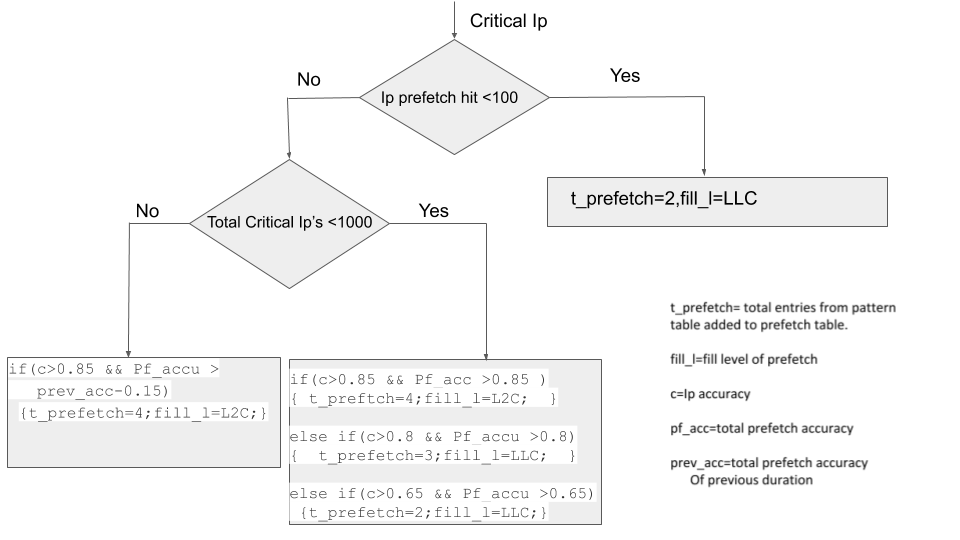
\includegraphics[scale=0.45]{images/Less_Band.png}}\par\medskip
\caption{SPP with low bandwidth consumption}
\label{fig:lessbw}
\end{figure}

\section{Prediction using Global Prefetch Accuracy}

We have already discussed how local prefetch accuracy per IP can be used to decide prefetch lookahead.
Another parameter we can use in deciding 
lookahead depth is the global accuracy of prefetching at various levels of the cache hierarchy and the overall accuracy
of the prefetcher. IP-based prefetch accuracy is a local parameter and it does not take into account the overall reaction
of the system to prefetching. Also, we need some parameter to check if a particular cache level is getting polluted due to aggressive prefetching.
It is always desirable to have the most frequently used data in the inner levels of the cache hierarchy. However, since the
inner level caches are also small in size, they can easily become polluted. At LLC we can have
more prefetched data, but it is also shared. So, we also need to take that into account.

We have measured prefetch accuracy at level 2 cache (L2C), at the last level of cache (LLC) and the overall prefetch accuracy. We also keep resetting
these accuracy counters at regular intervals so that they carry results of the recent history.
SPP has a thresholding mechanism for every prefetch by which it decides at which level of the cache hierarchy the prefetch will be inserted. So, according to the prefertch accuracy of the cache levels, we can adjust
this fill level. For example, if the accuracy of L2C goes down, we can stop prefetching to this level and
insert the prefetches into LLC only.
As with other parameters, deciding a threshold value for the accuracy is again a critical task. This
requires multiple simulations. We find that a combination of local IP accuracy and global prefetch accuracy is desirable.

\section{Deciding Fill Level of Prefetches}

As discussed earlier, SPP prefetches into two different cache levels depending upon the threshold values of the confidence. These two thresholds are Prefetch Threshold (PF\_Threshold) and Fill
Threshold (FILL\_Threshold). If the confidence of a prefetch is greater than the fill threshold, it is inserted
into L2C and LLC; if it is greater than the Prefetch Threshold, it is inserted in the LLC only;
if it is less than the prefetch threshold, it is not prefetched.

For the critical loads, we do not depend on the SPP confidence to decide the level of the prefetches. Instead,
we use parameters like IP-based local accuracy and the overall prefetch accuracy for this. We starts with an aggressive scheme inserting most of the prefetches into L2C and LLC. After the initial phase, all
parameters start getting enough training data so that we can make predictions based on them.
It is observed that most of the time L2C has high prefetch accuracy~(above 90\%) and
LLC has around 50\% to 60\% prefetch accuracy. This is because most of the time, prefetched blocks are present in L2C and they receive demand hits. The prefetched blocks which are in the LLC do not get hits most of the time and get
replaced by other blocks.
Decision of the fill level of the prefetch is most critical to performance because prefetching a good
number of accurate prefetches into the L2C significantly boosts the performance of the system.

\section{Periodic Updates of Parameters and Initialization}

As already discussed, there are multiple parameters like prefetch accuracy, ROB head stall, etc. that we need to keep track of at run-time. 
These parameters need to capture the behaviour of every phase of the workload to have an effective impact on
performance. It is done by dividing the program or workload execution into multiple phases
based on some parameters like count of critical prefetches.
Once we decide this parameter, we need to decide the total length of the interval. Interval
length is decided empirically by running multiple simulations with different lengths. Interval length of 1000 critical prefetches is observed to be effective.

\section{Dynamic Thresholds}

As we have pointed out, we need to manage two thresholds, namely Fill and Prefetch thresholds that decide which level an incoming
prefetched block to insert into. In SPP, these thresholds are fixed to values of 90 and 25. We changed these
thresholds to different values and found out that we could get better accuracy by changing these
thresholds.
As we know, having more accurate prefetches in the L2C can significantly improve
performance. So we tried to decrease FILL\_Threshold to allow more prefetches at L2C
and increase PF\_Threshold to discard some useless prefetches.
This resulted in increased IPC with almost the same LLC bandwidth and increased L2C bandwidth.

We also tried to dynamically adjust these thresholds based on L2C and LLC prefetch accuracy. We
tried to increase or decrease these values based on the corresponding accuracy, but found out that these
thresholds saturate to their extreme values and result in the same effect as static thresholds.
For critical loads, we have two options. One option is to use SPP's inherent prediction mechanism and other
is to use our own lookahead prediction mechanism. A possible third way is to use SPP lookahead mechanism
for those workloads which have threshold at least equal to PF\_THRESHOLD and our own prediction mechanism
for those workloads which have threshold less than PF\_THRESHOLD. This will ensure that all
critical loads get lookahead depths with minimum pollution.
But if we need a more aggressive prefetcher we can assign it using our own predictions. But
aggressive prefetching will consume lots of cache as well as DRAM bandwidth. So, there is a tradeoff
between the two.

\section{Depth-wise and Total Prefetch-wise Approaches}

There are various ways we can change the total number of prefetches based on the prediction by the prefetcher.
One way is to control the total number of prefetches generated by the prefetcher and the other is to control the prefetch depth, which will indirectly control the prefetch count. In the SPP's pattern table, there are multiple entries depending upon the ways of it. We select entries from the pattern table depending upon various parameters for every depth given a critical IP. So, we basically select a subset of prefetches suggested by SPP if confidence generated by SPP is less than PF\_THRESHOLD and give them new confidence; otherwise it uses confidence as in SPP and prefetches same as SPP.
This results in performance almost same as SPP with less bandwidth consumption. In this low bandwidth version, to decide the threshold for fill level, we use IP-based local accuracy and overall prefetch accuracy, which every time is compared to the previous (interval)-(offset) to get the dynamic estimates.
We also prefetch into the LLC alone in the case when the number of critical IPs seen so far is less than 1000 to initialize and train all the parameters properly. Controlling the depth results in aggressive prefetching because at every depth we prefetch two or more blocks depending upon the number of ways in the SPP pattern table. We go beyond the depths used by SPP. In this version, we directly put the prefetches in the L2C to get the more aggresive prefetching and use a threshold on IP-based and L2C accuracy to decide depth of prefetching. Controlling the number of prefetches is difficult but results in less bandwidth consumption and less aggressive prefetching compared to controlling depth. Our depth prediction mechanism integrated with SPP is shown in Figure~\ref{fig:sppdepth}.
\begin{figure}[H]
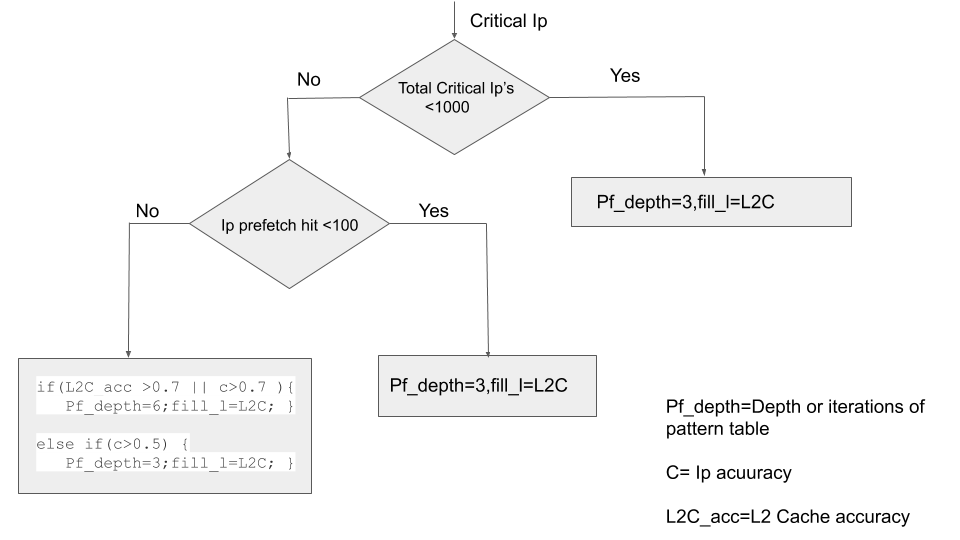
\includegraphics[scale=0.4]{images/Depth.png}
\caption{SPP with depth prediction configuration}
\label{fig:sppdepth}
\end{figure}

We have done experiments with different depths and with prediction of the number of prefetches. By
Varying depths, we observe that increasing depth increases bandwidth consumption and IPC up to a certain point
after which it starts decreasing due to bandwidth constraints.
This analysis help us in various ways. First,it shows the effect of prefetching at
various degrees (from less aggressive to more aggressive). Along with that, we are able to learn the effect of pollution at various cache levels and their effect on performance.